\chapter{Случайные векторы.}

\section*{Задачи 18.397, 18.398, 18.399}

Число $X$ выбирается случайным образом из множества целых чисел $\left \{ 1, 2, 3 \right \}$. Затем из того же множества выбирается наудачу число $Y$, большее первого
или равное ему. Требуется
\begin{enumerate}
    \item описать закон распределения случайного вектора $\left ( X, Y \right )$,
    \item построить функцию распределения вектора $(X, Y)$,
    \item описать закон распределения случайной величины $X$,
    \item описать закон распределения случайной величины $Y$,
    \item определить независимы или зависимы случайные величины $X$ и $Y$,
    \item вычислить математическое ожидание случайной величины $X$,
    \item вычислить математическое ожидание случайной величины $Y$,
    \item вычислить ковариационную матрицу случайных величин $X$ и $Y$,
    \item вычислить коэффициент корреляции случайных величин $X$ и $Y$,
    \item вычислить условное распределение $P_{\condition{X}{Y}}(x,y)$,
    \item вычислить условное математическое ожидание $\expectation{\condition{X}{Y}}$.
\end{enumerate}

\subsection*{Решение}
\begin{enumerate}
    \item Прежде всего необходимо выделить элементарные исходы эксперимента, определить их вероятности и значения величин $X$ и $Y$:

    \begin{tabular}{|p{5cm}|p{1cm}|p{1cm}|p{3cm}|}
        \hline
        Элементарное событие, $\omega_i$ & $X \left ( \omega_i \right )$ & $Y \left ( \omega_i \right )$
        & Вероятность
        \\
        \hline
        \hline
        $\omega_1$ & 1 & 1 & $\frac{1}{3} \cdot \frac{1}{3} = \frac{1}{9}$ \\
        \hline
        $\omega_2$ & 1 & 2 & $\frac{1}{3} \cdot \frac{1}{3} = \frac{1}{9}$ \\
        \hline
        $\omega_3$ & 1 & 3 & $\frac{1}{3} \cdot \frac{1}{3} = \frac{1}{9}$ \\
        \hline
        $\omega_4$ & 2 & 2 & $\frac{1}{3} \cdot \frac{1}{2} = \frac{1}{6}$ \\
        \hline
        $\omega_5$ & 2 & 3 & $\frac{1}{3} \cdot \frac{1}{2} = \frac{1}{6}$ \\
        \hline
        $\omega_6$ & 3 & 3 & $\frac{1}{3} \cdot 1 = \frac{1}{3}$           \\
        \hline
    \end{tabular}

    Последние три столбца описывают распределение вектора $\left ( X, Y \right )$.

    \item Пусть $F_{XY}(x, y)$ --- функция распределения двумерной случайной величины $(X, Y)$:
    \begin{equation}
        F_{XY}(x, y)
        = \probability{X < x, Y < y}
        = \sum_{(a, b) : a < x, b < y} \probability{X=a, Y=b}
    \end{equation}

    Например, вычислим значение функции распределения в точке $\left (1.5, 2.3 \right )$:
    \begin{equation}
        F_{XY}(1.5, 2.3) = \probability{X=1, Y=1} + \probability{X=1, Y=2} = \frac{1}{9} + \frac{1}{9} = \frac{2}{9}
    \end{equation}

    График функции распределения представлен на рисунке \ref{397:probability-function}.

    \begin{figure}[ht]
        \centering
        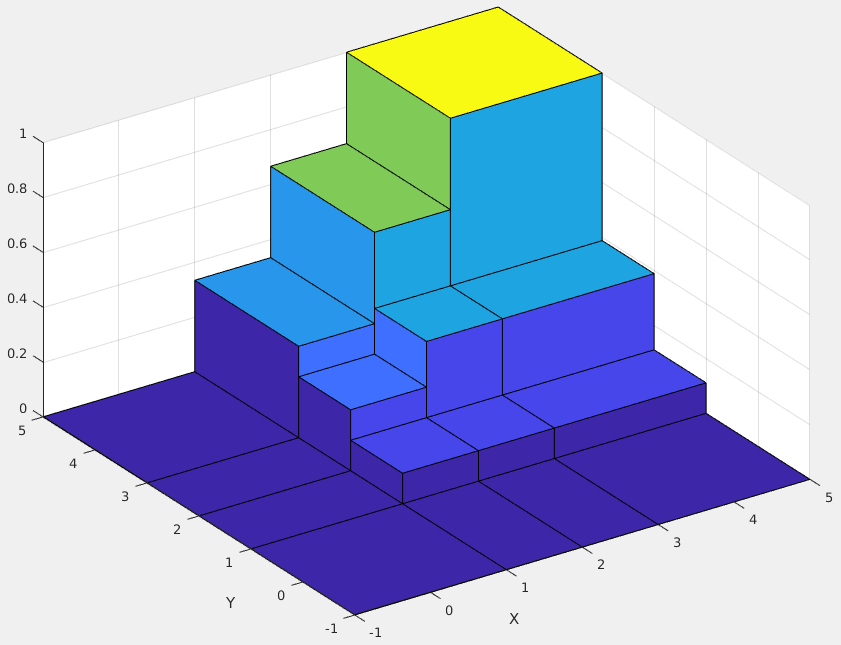
\includegraphics[width=0.6\textwidth]{lesson-9/397-probability-function.jpg}
        \caption{График функции распределения $F_{XY}(x,y)$.}
        \label{397:probability-function}
    \end{figure}

    \item Распределение случайной величины $X$ получается фиксированием значения величины $X$ и суммирования по всем возможным значениям случайной величины $Y$:
    \begin{equation}
        P\event{X = a} = \sum_{y} \probability{X=a, Y=y}
    \end{equation}
    Вычисляем вероятности:
    \begin{align}
        \probability{X=1} = & \probability{X=1,Y=1} + \probability{X=1,Y=2} + \probability{X=1,Y=3} = \frac{3}{9} = \frac{1}{3} \\
        \probability{X=2} = & \probability{X=2,Y=2} + \probability{X=2,Y=3} = \frac{2}{6} = \frac{1}{3} \\
        \probability{X=3} = & \probability{X=3,Y=3} = \frac{1}{3}
    \end{align}

    Записываем в таблицу значения и вероятности для случайной величины $X$:

    \begin{tabular}{|p{1cm}|p{1cm}|p{1cm}|p{1cm}|}
        \hline
        $x_i$ & 1             & 2             & 3             \\
        \hline
        $p_i$ & $\frac{1}{3}$ & $\frac{1}{3}$ & $\frac{1}{3}$ \\
        \hline
    \end{tabular}

    Если вычисления выполнены верно, то \textbf{сумма вероятностей равна 1}.

    \item Аналогично для случайной величины $Y$ вычисляем вероятности:
    \begin{align}
        \probability{Y=1} = & \probability{X=1, Y=1} = \frac{1}{9} = \frac{2}{18} , \\
        \probability{Y=2} = & \probability{X=1, Y=2} + \probability{X=2, Y=2} = \frac{1}{9} + \frac{1}{6} = \frac{5}{18} , \\
        \probability{Y=3} = & \probability{X=1, Y=3} + \probability{X=2, Y=3} + \probability{X=3, Y=3} = \frac{1}{9} + \frac{1}{6} + \frac{1}{3} = \frac{11}{18}
    \end{align}

    Записываем в таблицу значения и вероятности для случайной величины $Y$:

    \begin{tabular}{|p{1cm}|p{1cm}|p{1cm}|p{1cm}|}
        \hline
        $y_i$ & 1              & 2              & 3               \\
        \hline
        $p_i$ & $\frac{2}{18}$ & $\frac{5}{18}$ & $\frac{11}{18}$ \\
        \hline
    \end{tabular}

    \item Случайные величины являются независимыми, если:
    \begin{equation}
        F_{XY}(x,y) = F_X(x) \cdot F_Y(y),
    \end{equation}
    где $F_X(x)$ и $F_Y(y)$ --- функции распределения случайных величин $X$ и $Y$.

    Для дискретных случайных величин достаточно независимости событий $\event{X=a}$ и $\event{Y=b}$ при всех возможных $a$ и $b$:
    \begin{equation}
        \probability{X=a, Y=b} = \probability{X=a} \probability{Y=b}.
    \end{equation}

    Для проверки зависимости/независимости последовательно перебираем все возможные пары значений $(a, b)$ двумерной случайной величины $(X, Y)$:

    \begin{tabular}{|p{1cm}|p{1cm}|p{3cm}|p{2cm}|p{2cm}|p{5cm}|}
        \hline
        $a$ & $b$ & $\probability{X=a, Y=b}$ & $\probability{X=a}$ & $\probability{Y=b}$ & $\probability{X=a} \cdot \probability{Y=b}$ \\
        \hline
        1   & 1   & $\frac{1}{9}$            & $\frac{1}{3}$       & $\frac{1}{9}$       & $\frac{1}{27}$                              \\
        \hline
    \end{tabular}

    Дальше можно не проверять, поскольку уже не получено равенство:
    \begin{equation}
        \probability{X=1, Y=1} \neq \probability{X=1} \cdot \probability{Y=1} .
    \end{equation}
    поэтому случайные величины $X$ и $Y$ \textbf{зависимы}.

    \item Вычисляем математическое ожидание случайной величины $X$, используя полученный ранее закон распределения $X$:
    \begin{multline}
        \expectation{X} = \sum_{i=1}^3 x_i \cdot \probability{X=x_i}
        = 1 \cdot \probability{X=1} + 2 \cdot \probability{X=2} + 3 \cdot \probability{X=3} = \\
        %
        = 1 \cdot \frac{1}{3} + 2 \cdot \frac{1}{3} + 3 \cdot \frac{1}{3}
        = \frac{6}{3} = 2
        .
    \end{multline}

    \item Вычисляем математическое ожидание случайной величины $Y$, используя полученный ранее закон распределения $Y$:
    \begin{multline}
        \expectation{Y} = \sum_{i=1}^3 y_i \cdot \probability{Y=y_i}
        = 1 \cdot \probability{Y=1} + 2 \cdot \probability{Y=2} + 3 \cdot \probability{Y=3} = \\
        %
        = 1 \cdot \frac{2}{18} + 2 \cdot \frac{5}{18} + 3 \cdot \frac{11}{18}
        = \frac{2 + 10 + 33}{18} = \frac{45}{18} = \frac{5}{2} = 2.5
        .
    \end{multline}

    \item Ковариацией величин $X$ и $Y$ называется величина:
    \begin{equation}
        \covariance{X}{Y} = \expectation{\left ( X - \expectation{X} \right ) \left ( Y - \expectation{Y} \right )}
    \end{equation}
    Все возможные ковариации образуют ковариационную матрицу:
    \begin{equation}
        K =
        \begin{pmatrix}
            \covariance{X}{X} & \covariance{X}{Y} \\
            \covariance{Y}{X} & \covariance{Y}{Y}
        \end{pmatrix}
    \end{equation}
    Легко видеть, что
    \begin{equation}
        \covariance{X}{X}
        = \expectation{\left ( X - \expectation{X} \right ) \left ( Y - \expectation{Y} \right )}
        = \expectation{\left ( X - \expectation{X} \right )^2}
        = \variance{X}
    \end{equation}
    является дисперсией, поэтому на главной диагонали ковариационной матрицы стоят дисперсии величин:
    \begin{equation}
        K =
        \begin{pmatrix}
            \covariance{X}{X} & \covariance{X}{Y} \\
            \covariance{Y}{X} & \covariance{Y}{Y}
        \end{pmatrix}
        =
        \begin{pmatrix}
            \variance{X}      & \covariance{X}{Y} \\
            \covariance{Y}{X} & \variance{Y}
        \end{pmatrix}
    \end{equation}

    В силу свойства коммутативности:
    \begin{equation}
        \covariance{X}{Y}
        = \expectation{\left ( X - \expectation{X} \right ) \left ( Y - \expectation{Y} \right )}
        = \expectation{\left ( Y - \expectation{Y} \right ) \left ( X - \expectation{X} \right )}
        = \covariance{Y}{X} ,
    \end{equation}
    поэтому необходимо вычислить всего три величины: дисперсию случайной величины $X$
    \begin{multline}
        \variance{X}
        = \sum_{i=1}^3 \left ( x_i - \expectation{X} \right )^2 \cdot \probability{X=x_i} = \\
        %
        = ( 1 - 2 )^2 \cdot \probability{X=1} + ( 2 - 2 )^2 \cdot \probability{X=2} + ( 3 - 2 )^2 \cdot \probability{X=3} = \\
        %
        = 1^2 \cdot \frac{1}{3} + 0 \cdot \frac{1}{3} + 1^2 \cdot \frac{1}{3} = \frac{2}{3},
    \end{multline}
    дисперсию случайной величины $Y$
    \begin{multline}
        \variance{Y}
        = \sum_{i=1}^3 \left ( y_i - \expectation{Y} \right )^2 \cdot \probability{Y=y_i} = \\
        = ( 1 - 2.5 )^2 \cdot \probability{Y=1} + ( 2 - 2.5 )^2 \cdot \probability{Y=2} + ( 3 - 2.5 )^2 \cdot \probability{Y=3} = \\
        %
        = 1.5^2 \cdot \frac{1}{9} + 0.5^2 \cdot \frac{5}{18} + 0.5^2 \cdot \frac{11}{18}
        = \frac{2.25 \cdot 2 + 0.25 \cdot 5 + 0.25 \cdot 11}{18} = \\
        %
        = \frac{4.5 + 1.25 + 2.75}{18}
        = \frac{8.5}{18}
    \end{multline}
    и ковариацию случайных величин $X$ и $Y$
    \begin{equation}
        \covariance{X}{Y} = \sum_{i=1}^3 \sum_{j=1}^3 \left ( x_i - \expectation{X} \right ) \left ( y_j - \expectation{Y} \right ) \cdot \probability{X=x_i, Y=y_j}
    \end{equation}

    Запишем вычисления в таблицу:

    \begin{tabular}{|p{1cm}|p{1cm}|p{4cm}|p{8cm}|}
        \hline
        $x_i$ & $y_i$ & $\probability{X=x_i, Y=y_i}$ & $\left ( x_i - \expectation{X} \right ) \left ( y_j - \expectation{Y} \right ) \cdot \probability{X=x_i, Y=y_j}$ \\
        \hline
        1     & 1     & $\frac{1}{9}$                & $( 1 - 2 ) ( 1 - 2.5 ) \frac{1}{9} = \frac{1.5}{9} = \frac{3}{18}$                                               \\
        \hline
        1     & 2     & $\frac{1}{9}$                & $( 1 - 2 ) ( 2 - 2.5 ) \frac{1}{9} = \frac{0.5}{9} = \frac{1}{18}$                                               \\
        \hline
        1     & 3     & $\frac{1}{9}$                & $( 1 - 2 ) ( 3 - 2.5 ) \frac{1}{9} = -\frac{0.5}{9} = - \frac{1}{18}$                                            \\
        \hline
        2     & 2     & $\frac{1}{6}$                & $( 2 - 2 ) ( 2 - 2.5 ) \frac{1}{6} = 0$                                                                          \\
        \hline
        2     & 3     & $\frac{1}{6}$                & $( 2 - 2 ) ( 3 - 2.5 ) \frac{1}{6} = 0$                                                                          \\
        \hline
        3     & 3     & $\frac{1}{3}$                & $( 3 - 2 ) ( 3 - 2.5 ) \frac{1}{3} = \frac{0.5}{3} = \frac{3}{18}$                                               \\
        \hline
    \end{tabular}

    Складывая числа в последнем столбце, получаем значение ковариации случайных величин $X$ и $Y$:
    \begin{equation}
        \covariance{X}{Y} = \frac{3}{18} + \frac{1}{18} - \frac{1}{18} + 0 + 0 + \frac{3}{18} = \frac{6}{18} = \frac{1}{3}
    \end{equation}

    Таким образом, ковариационная матрица имеет вид:
    \begin{equation}
        K =
        \begin{pmatrix}
            \frac{2}{3} & \frac{1}{3}    \\
            \frac{1}{3} & \frac{8.5}{18}
        \end{pmatrix}
    \end{equation}

    \item Коэффициент корреляции $\rho_{XY}$ случайных величин $X$ и $Y$ определяется равенством:
    \begin{equation}
        \rho_{XY}
        = \frac{\covariance{X}{Y}}{\sqrt{\variance{X} \variance{Y}}}
        = \frac{\frac{1}{3}}{\sqrt{\frac{2}{3} \cdot \frac{8.5}{18}}}
        = \frac{\frac{1}{3}}{\sqrt{\frac{1}{3} \cdot \frac{8.5}{9}}}
        = \frac{\frac{1}{3}}{\frac{1}{3} \sqrt{\frac{1}{3} \cdot 8.5}}
        = \frac{1}{\sqrt{\frac{8.5}{3}}}
        = \sqrt{\frac{3}{8.5}}
        \approx 0.5941
        .
    \end{equation}

%        \item Условное математическое ожидание --- это \textbf{случайная величина}, которая конструируется особым образом.
%
%        Нас интересует условное математическое ожидание $\expectation{\condition{X}{Y}}$ относительно $Y$, поэтому прежде всего нужно выделить те события,
%        которые являются различимыми на основе значений случайной величины $Y$:
%        \begin{equation}
%            \begin{array}{lcl}
%                Y=1 & : & A_1 = \left \{ \omega_1 \right \},                    \\
%                Y=2 & : & A_2 = \left \{ \omega_2, \omega_4 \right \},          \\
%                Y=3 & : & A_3 = \left \{ \omega_3, \omega_5, \omega_6 \right \}
%            \end{array}
%        \end{equation}
%        Если величина $Y$ принимает значение $2$, то мы знаем, что имеет место элементарный исход из множества $A_2$, но не знаем какой именно $\omega_2$ или $\omega_4$.
%        На основе значений $Y$ мы можем различать только три множества элементарных исходов, но в случаях $Y=2$ и $Y=3$ не можем точно указать элементарный исход.
%
%        На различимых множествах $A_i$ для всех элементарных исходов $\omega \in A_i$ случайная величина $\expectation{\condition{X}{Y}}$ может принимать только одно
%        постоянное значение --- не может изменяться в пределах одного множества $A_i$, поэтому необходимо найти три неизвестных числа, которые обозначим $a_i$:
%        \begin{equation}
%            \omega \in A_i \; : \; \expectation{\condition{X}{Y}}(\omega) = a_i
%        \end{equation}
%
%        Условное математическое ожидание $\expectation{\condition{X}{Y}}$ --- это что-то вроде проекции величины $X$ на множества, различимые с помощью величины $Y$,
%        "редуцирование"{} (упрощение, огрубление) величины $X$. Условное математическое ожидание $\expectation{\condition{X}{Y}}$ приближает в среднем величину $X$.
%
%        Числа $a_i$ определяются из равенств:
%        \begin{gather}
%            \sum_{\omega \in A_i} a_i \probability{\omega} = \sum_{\omega \in A_i} X(\omega) \probability{\omega} , \\
%            a_i \sum_{\omega \in A_i} \probability{\omega} = \sum_{\omega \in A_i} X(\omega) \probability{\omega} , \\
%            a_i \probability{A_i} = \sum_{\omega \in A_i} X(\omega) \probability{\omega} , \\
%            a_i = \frac{\sum_{\omega \in A_i} X(\omega) \probability{\omega}}{\probability{A_i}} \label{397:a_i_1}
%        \end{gather}
%        которые обозначают следущее: $a_i$ --- это среднее значение величины $X(\omega)$ на множестве $A_i$, отнесенное к вероятности множества $A_i$. Можно записать и так:
%        \begin{equation}
%            a_i = \sum_{\omega \in A_i} X(\omega) \frac{\probability{\omega}}{\probability{A_i}} \label{397:a_i_2}
%        \end{equation}
%        интерпретация будет следующей: $a_i$ --- это среднее значение величины $X(\omega)$ с учётом вклада каждого элементарного события $\omega_i$ в множество $A_i$.
%        Равенство \eqref{397:a_i_2} можно преобразовать далее, если суммировать не по элементарным событиям $\omega$, а по значениям $x$
%        величины $X$, которые встречаются на множестве $A_i$, для этого в множестве $A_i$ нужно выделить подмножества элементарных исходов
%        с одинаковыми значениями величины $X$:
%        \begin{multline}
%            \label{397:conditional}
%            a_i
%            = \sum_{\omega \in \event{Y=y_i}} X(\omega) \frac{\probability{\omega}}{\probability{\event{Y=y_i}}}
%            = \sum_{x_j} \sum_{\omega \in \event{X=x_j} \cap \event{Y=y_i}} X(\omega) \frac{\probability{\omega}}{\probability{Y=y_i}} = \\
%            %
%            = \sum_{x_j} \sum_{\omega \in \event{X=x_j} \cap \event{Y=y_i}} x_j \frac{\probability{\omega}}{\probability{Y=y_i}}
%            = \sum_{x_j} x_j \frac{\sum_{\omega \in \event{X=x_j} \cap \event{Y=y_i}} \probability{\omega}}{\probability{Y=y_i}} = \\
%            %
%            = \sum_{x_j} x_j \frac{\probability{X=x_j, Y=y_i}}{\probability{Y=y_i}} = \\
%            = \sum_{x_j} x_j \probability{\condition{X=x_j}{Y=y_i}} .
%        \end{multline}
%        Во многих учебниках можно встретить именно такую запись для вычисления значений условного математического ожидания.
%
%        При вычислении $\expectation{\condition{X}{Y}}$ я буду использовать равенство \eqref{397:a_i_1} (оно кажется более простым):
%        \begin{equation}
%            a_1
%            = \frac{X(\omega_1) \probability{\omega_1}}{\probability{A_1}}
%            = \frac{1 \cdot \frac{1}{9}}{\frac{1}{9}}
%            = 1
%        \end{equation}
%        \begin{multline}
%            a_2
%            = \frac{X(\omega_2) \probability{\omega_2} + X(\omega_4) \probability{\omega_4}}{\probability{A_2}}
%            = \frac{X(\omega_2) \probability{\omega_2} + X(\omega_4) \probability{\omega_4}}{\probability{\omega_2} + \probability{\omega_4}} = \\
%            %
%            = \frac{1 \frac{1}{9} + 2 \frac{1}{6}}{\frac{1}{9} + \frac{1}{6}}
%            = \frac{1 \cdot 2 + 2 \cdot 3}{2 + 3}
%            = \frac{8}{5}
%        \end{multline}
%        \begin{multline}
%            a_3
%            = \frac{X(\omega_3) \probability{\omega_3} + X(\omega_5) \probability{\omega_5} + X(\omega_6) \probability{\omega_6}}{\probability{A_3}} = \\
%            %
%            = \frac{X(\omega_3) \probability{\omega_3} + X(\omega_5) \probability{\omega_5} + X(\omega_6) \probability{\omega_6}}{\probability{\omega_3} + \probability{\omega_5} + \probability{\omega_6}} = \\
%            %
%            = \frac{1 \frac{1}{9} + 2 \frac{1}{6} + 3 \frac{1}{3}}{\frac{1}{9} + \frac{1}{6} + \frac{1}{3}}
%            = \frac{1 \cdot 2 + 2 \cdot 3 + 3 \cdot 6}{2 + 3 + 6}
%            = \frac{26}{11}
%        \end{multline}
%
%        Во многих задачах не требуют вычислять полностью условное математическог ожидание $\expectation{\condition{X}{Y}}$, а интересуются лишь одним
%        значением условного математического ожидания при значении $Y=y_i$. Нужно понимать, что это то значение $a_i$, которое условное математическое ожидание
%        принимает на множестве $A_i$. Иногда это значение $a_i$ записывают в виде $\expectation{\condition{X}{Y=y_i}}$. В данной задаче, например:
%        \begin{equation}
%            \expectation{\condition{X}{Y=3}} = \frac{26}{11}
%        \end{equation}

    \item Условное распределение $P_{\condition{X}{Y}}(x,y)$ принимает значения условных вероятностей событий вида $\event{X=x}$ относительно событий вида $\event{Y=y}$:
    \begin{equation}
        P_{\condition{X}{Y}}(x,y) = \frac{\probability{X=x, Y=y}}{\probability{Y=y}} .
    \end{equation}

    Для $Y=1$ условное распределение $X$:
    \begin{gather}
        P_{\condition{X}{Y}}(1,1)
        = \frac{\probability{X=1, Y=1}}{\probability{Y=1}}
        = \frac{\frac{1}{9}}{\frac{2}{18}}
        = \frac{\frac{1}{9}}{\frac{1}{9}}
        = 1 , \\
        %
        P_{\condition{X}{Y}}(2,1)
        = \frac{\probability{X=2, Y=1}}{\probability{Y=1}}
        = \frac{0}{\frac{2}{18}}
        = 0 , \\
        %
        P_{\condition{X}{Y}}(3,1)
        = \frac{\probability{X=3, Y=1}}{\probability{Y=1}}
        = \frac{0}{\frac{2}{18}}
        = 0 .
    \end{gather}

    Для $Y=2$ условное распределение $X$:
    \begin{gather}
        P_{\condition{X}{Y}}(1,2)
        = \frac{\probability{X=1, Y=2}}{\probability{Y=2}}
        = \frac{\frac{1}{9}}{\frac{5}{18}}
        = \frac{2}{5} , \\
        %
        P_{\condition{X}{Y}}(2,2)
        = \frac{\probability{X=2, Y=2}}{\probability{Y=2}}
        = \frac{\frac{1}{6}}{\frac{5}{18}}
        = \frac{3}{5} , \\
        %
        P_{\condition{X}{Y}}(3,2)
        = \frac{\probability{X=3, Y=2}}{\probability{Y=2}}
        = \frac{0}{\frac{5}{18}}
        = 0 .
    \end{gather}

    Для $Y=3$ условное распределение $X$:
    \begin{gather}
        P_{\condition{X}{Y}}(1,3)
        = \frac{\probability{X=1, Y=3}}{\probability{Y=3}}
        = \frac{\frac{1}{9}}{\frac{11}{18}}
        = \frac{2}{11} , \\
        %
        P_{\condition{X}{Y}}(2,3)
        = \frac{\probability{X=2, Y=3}}{\probability{Y=3}}
        = \frac{\frac{1}{6}}{\frac{11}{18}}
        = \frac{3}{11} , \\
        %
        P_{\condition{X}{Y}}(3,3)
        = \frac{\probability{X=3,Y=3}}{\probability{Y=3}}
        = \frac{\frac{1}{3}}{\frac{11}{18}}
        = \frac{6}{11} .
    \end{gather}

    Условное распределение $X$ изменяется в зависимости от распределения $Y$ (случайные величины зависимы).

    Для $Y=1$:

    \begin{tabular}{|p{3cm}|p{1cm}|p{1cm}|p{1cm}|}
        \hline
        $x$                          & 1 & 2 & 3 \\
        \hline
        $P_{\condition{X}{Y}}(x, 1)$ & 1 & 0 & 0 \\
        \hline
    \end{tabular}

    Для $Y=2$:

    \begin{tabular}{|p{3cm}|p{1cm}|p{1cm}|p{1cm}|}
        \hline
        $x$                          & 1             & 2             & 3 \\
        \hline
        $P_{\condition{X}{Y}}(x, 2)$ & $\frac{2}{5}$ & $\frac{3}{5}$ & 0 \\
        \hline
    \end{tabular}

    Для $Y=3$:

    \begin{tabular}{|p{3cm}|p{1cm}|p{1cm}|p{1cm}|}
        \hline
        $x$                          & 1              & 2              & 3              \\
        \hline
        $P_{\condition{X}{Y}}(x, 3)$ & $\frac{2}{11}$ & $\frac{3}{11}$ & $\frac{6}{11}$ \\
        \hline
    \end{tabular}

    Для условного распределения $P_{\condition{X}{Y}}(x,y)$ при фиксированном значении $y$ выполняется условие нормировки ---
    \textbf{сумма условных вероятностей равна 1}, например:
    \begin{equation}
        P_{\condition{X}{Y}}(1,3) + P_{\condition{X}{Y}}(2,3) + P_{\condition{X}{Y}}(3,3)
        = \frac{2}{11} + \frac{3}{11} + \frac{6}{11}
        = 1 .
    \end{equation}

    \item Значения условного математического ожидания вычисляются с помощью условного распределения $P_{\condition{X}{Y}}(x,y)$:
    \begin{equation}
        \expectation{\condition{X}{Y=y}} = \sum_{x_i} x_i P_{\condition{X}{Y}}(x_i, y)
    \end{equation}

    Для $Y=1$:
    \begin{multline}
        \expectation{\condition{X}{Y=1}}
        = \sum_{x=1}^3 x \cdot P_{\condition{X}{Y}}(x, 1) = \\
        %
        = 1 \cdot P_{\condition{X}{Y}}(1, 1) + 2 \cdot P_{\condition{X}{Y}}(2, 1) + 3 \cdot P_{\condition{X}{Y}}(3, 1)
        = 1 \cdot 1 + 2 \cdot 0 + 3 \cdot 0
        = 1
    \end{multline}

    Для $Y=2$:
    \begin{multline}
        \expectation{\condition{X}{Y=2}}
        = \sum_{x=1}^3 x \cdot P_{\condition{X}{Y}}(x, 2) = \\
        %
        = 1 \cdot P_{\condition{X}{Y}}(1, 2) + 2 \cdot P_{\condition{X}{Y}}(2, 2) + 3 \cdot P_{\condition{X}{Y}}(3, 2)
        = 1 \cdot \frac{2}{5} + 2 \cdot \frac{3}{5} + 3 \cdot 0
        = \frac{8}{5}
    \end{multline}

    Для $Y=3$:
    \begin{multline}
        \expectation{\condition{X}{Y=3}}
        = \sum_{x=1}^3 x \cdot P_{\condition{X}{Y}}(x, 3) = \\
        %
        = 1 \cdot P_{\condition{X}{Y}}(1, 3) + 2 \cdot P_{\condition{X}{Y}}(2, 3) + 3 \cdot P_{\condition{X}{Y}}(3, 3)
        = 1 \cdot \frac{2}{11} + 2 \cdot \frac{3}{11} + 3 \cdot \frac{6}{11}
        = \frac{2}{11} + \frac{6}{11} + \frac{18}{11}
        = \frac{26}{11} .
    \end{multline}

    \item Для математического ожидания величины $X$ справедливо равенство:
    \begin{equation}
        \expectation{X} = \expectation{\expectation{\condition{X}{Y}}} ,
    \end{equation}

    В данной задаче правая часть имеет вид:
    \begin{equation}
        \expectation{X} = \sum_{y=1}^3 \expectation{\condition{X}{Y=y}} \probability{Y=y}
    \end{equation}
    и является аналогом формулы полной вероятности: вычисление математического ожидания можно разбить на несколько более простых случаев.

    Вычислим правую часть
    \begin{multline}
        \expectation{X}
        = \sum_{y=1}^3 \expectation{\condition{X}{Y=y}} \probability{Y=y} = \\
        %
        = \expectation{\condition{X}{Y=1}} \probability{Y=1} + \expectation{\condition{X}{Y=2}} \probability{Y=2} + \expectation{\condition{X}{Y=3}} \probability{Y=3} = \\
        %
        = 1 \cdot \frac{2}{18} + \frac{8}{5} \cdot \frac{5}{18}  + \frac{26}{11} \cdot \frac{11}{18}
        = \frac{2 + 8 + 26}{18}
        = \frac{36}{18}
        = 2
    \end{multline}
\end{enumerate}

\subsection*{Ответ}
\begin{enumerate}
    \item закон распределения случайного вектора $\left ( X, Y \right )$:

    \begin{tabular}{|p{1cm}|p{1cm}|p{3cm}|}
        \hline
        $X$ & $Y$ & Вероятность                                   \\
        \hline
        \hline
        1   & 1   & $\frac{1}{3} \cdot \frac{1}{3} = \frac{1}{9}$ \\
        \hline
        1   & 2   & $\frac{1}{3} \cdot \frac{1}{3} = \frac{1}{9}$ \\
        \hline
        1   & 3   & $\frac{1}{3} \cdot \frac{1}{3} = \frac{1}{9}$ \\
        \hline
        2   & 2   & $\frac{1}{3} \cdot \frac{1}{2} = \frac{1}{6}$ \\
        \hline
        2   & 3   & $\frac{1}{3} \cdot \frac{1}{2} = \frac{1}{6}$ \\
        \hline
        3   & 3   & $\frac{1}{3} \cdot 1 = \frac{1}{3}$           \\
        \hline
    \end{tabular}

    \item закон распределения случайной величины $X$:

    \begin{tabular}{|p{1cm}|p{1cm}|p{1cm}|p{1cm}|}
        \hline
        $x_i$ & 1             & 2             & 3             \\
        \hline
        $p_i$ & $\frac{1}{3}$ & $\frac{1}{3}$ & $\frac{1}{3}$ \\
        \hline
    \end{tabular}

    \item закон распределения случайной величины $Y$:

    \begin{tabular}{|p{1cm}|p{1cm}|p{1cm}|p{1cm}|}
        \hline
        $y_i$ & 1              & 2              & 3               \\
        \hline
        $p_i$ & $\frac{2}{18}$ & $\frac{5}{18}$ & $\frac{11}{18}$ \\
        \hline
    \end{tabular}

    \item величины $X$ и $Y$ зависимы,
    \item математическое ожидание случайной величины $X$: 2,
    \item математическое ожидание случайной величины $Y$: 2.5,
    \item ковариационная матрица вектора $\left ( X, Y \right )$:
    $
    \begin{pmatrix}
        \frac{2}{3} & \frac{1}{3}    \\
        \frac{1}{3} & \frac{8.5}{18}
    \end{pmatrix}
    $

    \item коэффициент корреляции случайных величин $X$ и $Y$: $\sqrt{\frac{3}{8.5}} \approx 0.5941$,
    \item условное распределение:

    Для $Y=1$:

    \begin{tabular}{|p{3cm}|p{1cm}|p{1cm}|p{1cm}|}
        \hline
        $x$                          & 1 & 2 & 3 \\
        \hline
        $P_{\condition{X}{Y}}(x, 1)$ & 1 & 0 & 0 \\
        \hline
    \end{tabular}

    Для $Y=2$:

    \begin{tabular}{|p{3cm}|p{1cm}|p{1cm}|p{1cm}|}
        \hline
        $x$                          & 1             & 2             & 3 \\
        \hline
        $P_{\condition{X}{Y}}(x, 2)$ & $\frac{2}{5}$ & $\frac{3}{5}$ & 0 \\
        \hline
    \end{tabular}

    Для $Y=3$:

    \begin{tabular}{|p{3cm}|p{1cm}|p{1cm}|p{1cm}|}
        \hline
        $x$                          & 1              & 2              & 3              \\
        \hline
        $P_{\condition{X}{Y}}(x, 3)$ & $\frac{2}{11}$ & $\frac{3}{11}$ & $\frac{6}{11}$ \\
        \hline
    \end{tabular}

    \item условное математическое ожидание:
    \begin{gather*}
        \expectation{\condition{X}{Y=1}} = 1 , \\
        \expectation{\condition{X}{Y=2}} = \frac{8}{5} , \\
        \expectation{\condition{X}{Y=3}} = \frac{26}{11} .
    \end{gather*}
\end{enumerate}


\section*{Задачи 18.404, 18.405, 18.406}

Плотность распределения вероятностей случайного вектора $\left ( X, Y \right )$ имеет следующий вид:
$$
f_{X,Y}(x,y)
= \left \{
\begin{array}{ll}
    c ( x + y ), & 0 \le x \le 1, 0 \le y \le 1 \\
    0,           & \text{в остальных случаях}
\end{array}
\right .
.
$$
Требуется:
\begin{enumerate}
    \item определить константу $c$,
    \item вычислить функцию распределения $F_{X,Y}(x,y)$,
    \item вычислить вероятность $\probability{X + Y < 1}$,
    \item найти безусловную плотность вероятности $f_X(x)$ величины $X$,
    \item определить зависимы или независимы случайные величины $X$ и $Y$,
    \item найти центр рассеивания --- математические ожидания $\expectation{X}$ и $\expectation{Y}$,
    \item вычислить ковариационную матрицу $K_{X,Y}$ величин $X$ и $Y$.
    \item найти условную плотность вероятности $f_{\condition{X}{Y}}(x,y)$ распределения $X$ относительно $Y$,
    \item вычислить условное математическое ожидание $\expectation{\condition{X}{Y}}$.
\end{enumerate}

\subsection*{Решение}
\begin{enumerate}
    \item Констата $c$ определяется условием нормировки:
    \begin{gather}
        \int \limits_{-\infty}^{\infty} \int \limits_{-\infty}^{\infty} f_{X,Y}(x,y) dx dy = 1 , \\
        \int \limits_{0}^{1} \int \limits_{0}^{1} c ( x + y ) dx dy = 1 , \\
        c \int \limits_{0}^{1} \int \limits_{0}^{1} ( x + y ) dx dy = 1 , \\
        c \int \limits_{0}^{1} \left . \left ( \frac{x^2}{2} + x y \right ) \right |_0^1 dy = 1 , \\
        c \int \limits_{0}^{1} \left ( \frac{1}{2} + y \right ) dy = 1 , \\
        c \left . \left ( \frac{1}{2} y + \frac{y^2}{2} \right ) \right |_0^1 = 1 , \\
        c \left ( \frac{1}{2} + \frac{1}{2} \right ) = 1 , \\
        c = 1 .
    \end{gather}

    \item Совместная функция распределения $F_{X,Y}(x,y)$ определяется равенством:
    \begin{multline}
        F_{X,Y}(x,y)
        = \int \limits_{-\infty}^x \int \limits_{-\infty}^y f_{X,Y}(u,v) dv du
        = \left \{
        \begin{array}{ll}
            0 ,                                                 & x < 0 \text{ или } y < 0 ,     \\
            \int \limits_0^x \int \limits_0^y ( u + v ) dv du , & 0 \le x \le 1, 0 \le y \le 1 , \\
            \int \limits_0^x \int \limits_0^1 ( u + v ) dv du , & 0 \le x \le 1, 1 < y ,         \\
            \int \limits_0^1 \int \limits_0^y ( u + v ) dv du , & 1 < x, 0 \le y \le 1 ,         \\
            \int \limits_0^1 \int \limits_0^1 ( u + v ) dv du , & 1 < x, 1 < y
        \end{array}
        \right .
    \end{multline}

    \begin{figure}[h]
        \centering
        \begin{subfigure}{0.3\textwidth}
            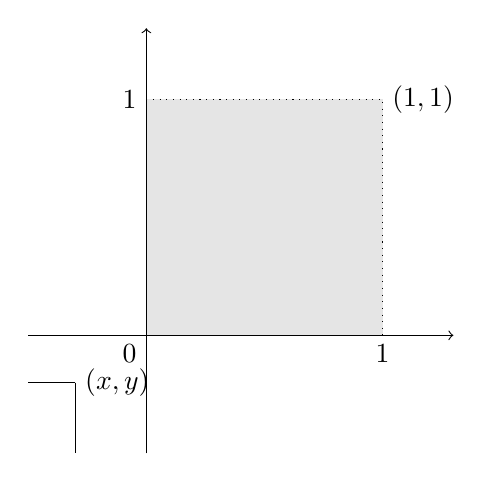
\begin{tikzpicture}[scale=3]
% прямоугольники
                \fill [fill=gray!20] ( 0, 0 ) -- ( 0, 1 ) -- ( 1, 1 ) -- ( 1, 0 );
% оси
                \draw [->] ( -0.5, 0 ) -- ( 1.3, 0 );
                \draw [->] ( 0, -0.5 ) -- ( 0, 1.3 );

% квадратик
                \draw [dotted] ( 0, 1 ) -- ( 1, 1 ) -- ( 1, 0 );
                \node [below left] at ( 0, 0 ) {$0$};
                \node [left] at ( 0, 1 ) {$1$};
                \node [right] at ( 1, 1 ) {$(1,1)$};
                \node [below] at ( 1, 0 ) {$1$};
% угольник
                \draw ( -0.3, -0.2 ) -- ( -0.3, -0.5 );
                \draw ( -0.3, -0.2 ) -- ( -0.5, -0.2 );
                \node [right] at ( -0.3, -0.2 ) {$(x,y)$};
            \end{tikzpicture}
        \end{subfigure}
        \hfill
        \begin{subfigure}{0.3\textwidth}
            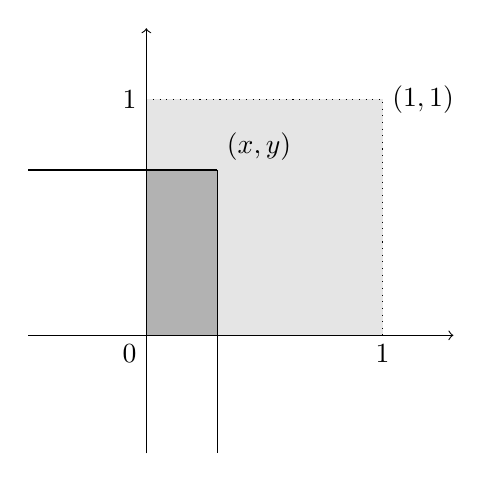
\begin{tikzpicture}[scale=3]
% прямоугольники
                \fill [fill=gray!20] ( 0, 0 ) -- ( 0, 1 ) -- ( 1, 1 ) -- ( 1, 0 );
                \fill [fill=gray!60] ( 0, 0 ) -- ( 0, 0.7 ) -- ( 0.3, 0.7 ) -- ( 0.3, 0 );

% оси
                \draw [->] ( -0.5, 0 ) -- ( 1.3, 0 );
                \draw [->] ( 0, -0.5 ) -- ( 0, 1.3 );

% квадратик
                \draw [dotted] ( 0, 1 ) -- ( 1, 1 ) -- ( 1, 0 );
                \node [below left] at ( 0, 0 ) {$0$};
                \node [left] at ( 0, 1 ) {$1$};
                \node [right] at ( 1, 1 ) {$(1,1)$};
                \node [below] at ( 1, 0 ) {$1$};
% угольник
                \draw ( 0.3, 0.7 ) -- ( 0.3, -0.5 );
                \draw ( 0.3, 0.7 ) -- ( -0.5, 0.7 );
                \node [above right] at ( 0.3, 0.7 ) {$(x,y)$};
            \end{tikzpicture}
        \end{subfigure}
        \hfill
        \begin{subfigure}{0.3\textwidth}
            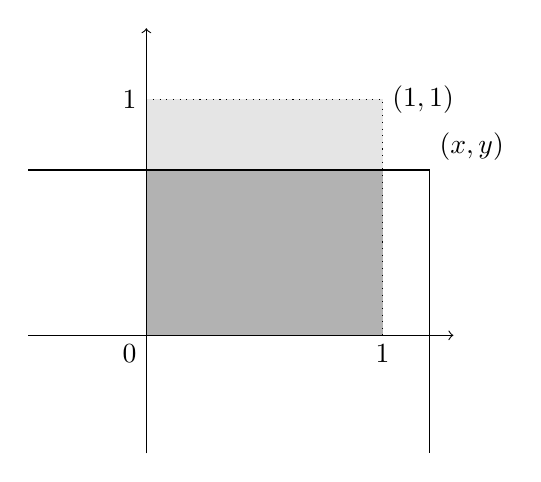
\begin{tikzpicture}[scale=3]
% прямоугольники
                \fill [fill=gray!20] ( 0, 0 ) -- ( 0, 1 ) -- ( 1, 1 ) -- ( 1, 0 );
                \fill [fill=gray!60] ( 0, 0 ) -- ( 0, 0.7 ) -- ( 1, 0.7 ) -- ( 1, 0 );

% оси
                \draw [->] ( -0.5, 0 ) -- ( 1.3, 0 );
                \draw [->] ( 0, -0.5 ) -- ( 0, 1.3 );

% квадратик
                \draw [dotted] ( 0, 1 ) -- ( 1, 1 ) -- ( 1, 0 );
                \node [below left] at ( 0, 0 ) {$0$};
                \node [left] at ( 0, 1 ) {$1$};
                \node [right] at ( 1, 1 ) {$(1,1)$};
                \node [below] at ( 1, 0 ) {$1$};
% угольник
                \draw ( 1.2, 0.7 ) -- ( 1.2, -0.5 );
                \draw ( 1.2, 0.7 ) -- ( -0.5, 0.7 );
                \node [above right] at ( 1.2, 0.7 ) {$(x,y)$};
            \end{tikzpicture}
        \end{subfigure}
        \caption{Вычисление функции распределения $F_{X,Y}(x,y)$.}
    \end{figure}

    Вычисляем интегралы:
    \begin{multline}
        \int \limits_0^x \int \limits_0^y ( u + v ) dv du
        = \int \limits_0^x \left . \left ( u v + \frac{v^2}{2} \right ) \right |_0^y du
        = \int \limits_0^x \left ( u y + \frac{y^2}{2} \right ) du = \\
%
        = \left . \left ( \frac{u^2}{2} y + u \frac{y^2}{2} \right ) \right |_0^x
        = \frac{x^2}{2} y + x \frac{y^2}{2}
    \end{multline}
    \begin{multline}
        \int \limits_0^x \int \limits_0^1 ( u + v ) dv du
        = \int \limits_0^x \left . \left ( u v + \frac{v^2}{2} \right ) \right |_0^1 du
        = \int \limits_0^x \left ( u + \frac{1}{2} \right ) du = \\
%
        = \left . \left ( \frac{u^2}{2} + u \frac{1}{2} \right ) \right |_0^x
        = \frac{x^2}{2} + \frac{x}{2}
    \end{multline}
    \begin{multline}
        \int \limits_0^1 \int \limits_0^y ( u + v ) dv du
        = \int \limits_0^1 \left . \left ( u v + \frac{v^2}{2} \right ) \right |_0^y du
        = \int \limits_0^1 \left ( u y + \frac{y^2}{2} \right ) du = \\
%
        = \left . \left ( \frac{u^2}{2} y + u \frac{y^2}{2} \right ) \right |_0^1
        = \frac{y}{2} + \frac{y^2}{2}
    \end{multline}
    Таким образом,
    \begin{equation}
        F_{X,Y}(x,y)
        = \left \{
        \begin{array}{ll}
            0 ,                                 & x < 0 \text{ или } y < 0 ,     \\
            \frac{x^2}{2} y + x \frac{y^2}{2} , & 0 \le x \le 1, 0 \le y \le 1 , \\
            \frac{x^2}{2} + \frac{x}{2} ,       & 0 \le x \le 1, 1 < y ,         \\
            \frac{y}{2} + \frac{y^2}{2} ,       & 1 < x, 0 \le y \le 1 ,         \\
            1 ,                                 & 1 < x, 1 < y
        \end{array}
        \right .
    \end{equation}

    \item Вероятность вычисляется интегрированием плотности вероятности:
    \begin{figure}[h]
        \center
        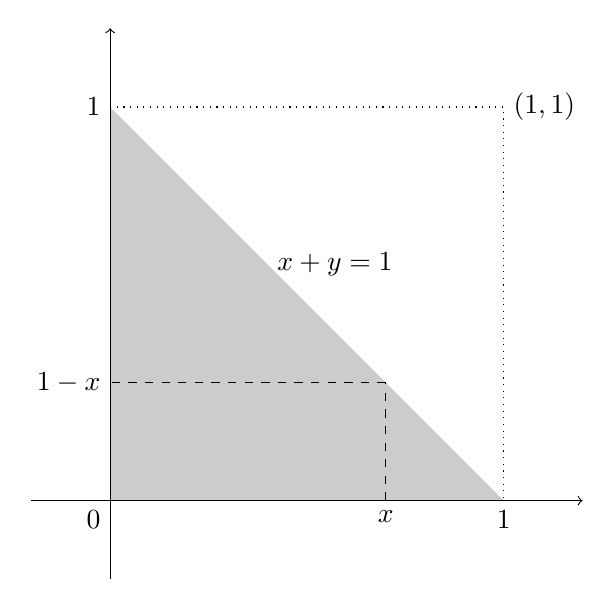
\begin{tikzpicture}[scale=5]
% треугольник
            \fill [fill=gray!40] ( 0, 0 ) -- ( 0, 1 ) -- ( 1, 0 );

% оси
            \draw [->] ( -0.2, 0 ) -- ( 1.2, 0 );
            \draw [->] ( 0, -0.2 ) -- ( 0, 1.2 );

% квадратик
            \draw [dotted] ( 0, 1 ) -- ( 1, 1 ) -- ( 1, 0 );
            \node [below left] at ( 0, 0 ) {$0$};
            \node [left] at ( 0, 1 ) {$1$};
            \node [right] at ( 1, 1 ) {$(1,1)$};
            \node [below] at ( 1, 0 ) {$1$};

% аргументы
            \draw [dashed] ( 0.7, 0 ) -- ( 0.7, 0.3 ) node [below] at ( 0.7, 0 ) {$x$};
            \draw [dashed] ( 0.7, 0.3 ) -- ( 0, 0.3 ) node [left] at ( 0, 0.3 ) {$1-x$};

            % прямая
            \node [right] at ( 0.4, 0.6 ) {$x+y=1$};
        \end{tikzpicture}
        \caption{Вычисление вероятности $\probability{X + Y < 1}$}
    \end{figure}

    \begin{multline}
        \probability{X + Y < 1}
        = \iint \limits_{x + y < 1} f_{X,Y}(x,y) dx dy
        = \int \limits_0^1 \int \limits_0^{1-x} (x+y) dy dx
        = \int \limits_0^1 \left . \left ( x y + \frac{y^2}{2} \right ) \right |_0^{1-x} dx = \\
%
        = \int \limits_0^1 \left ( x (1-x) + \frac{(1-x)^2}{2} \right ) dx
        = \int \limits_0^1 \left ( x - x^2 + \frac{1}{2} - x + \frac{1}{2} x^2 \right ) dx
        = \int \limits_0^1 \left ( \frac{1}{2} - \frac{1}{2} x^2 \right ) dx = \\
%
        = \frac{1}{2} \int \limits_0^1 \left ( 1 - x^2 \right ) dx
        = \frac{1}{2} \left . \left ( x - \frac{x^3}{3} \right ) \right |_0^1
        = \frac{1}{2} \left ( 1 - \frac{1}{3} \right )
        = \frac{1}{2} \cdot \frac{2}{3}
        = \frac{1}{3}
    \end{multline}

    \item Безусловyную плотность вероятности $f_X(x)$ величины $X$ можно вычислить с использованием плотности вероятности
    $f_{X,Y}(x,y)$ или функции распределения $F_{X,Y}(x,y)$.

    Вариант 1: интегрированием по $y$ плотности вероятности $f_{X,Y}(x,y)$.
    \begin{multline}
        f_X(x)
        = \int \limits_{-\infty}^{\infty} f_{X,Y}(x,y) dy
        =
        \left \{
        \begin{array}{ll}
            \int \limits_0^1 (x + y) dy, & 0 \le x \le 1              \\
            0,                           & \text{в остальных случаях}
        \end{array}
        \right . = \\
%
        =
        \left \{
        \begin{array}{ll}
            \left . \left ( x y + \frac{y^2}{2} \right ) \right |_0^1, & 0 \le x \le 1              \\
            0,                                                         & \text{в остальных случаях}
        \end{array}
        \right .
        =
        \left \{
        \begin{array}{ll}
            x + \frac{1}{2}, & 0 \le x \le 1              \\
            0,               & \text{в остальных случаях}
        \end{array}
        \right .
    \end{multline}

    Вариант 2: вычислением функции распределения $F_X(x)$ величины $X$ и дифференцированием.
    \begin{equation}
        F_X(x)
        = \lim_{y \rightarrow \infty} F_{X,Y}(x,y)
        = \left \{
        \begin{array}{ll}
            0,                           & x \le 0     \\
            \frac{x^2}{2} + \frac{x}{2}, & 0 < x \le 1 \\
            1,                           & 1 < x
        \end{array}
        \right .
    \end{equation}
    Плотность вероятности вычисляем с помощью производной:
    \begin{equation}
        f_X(x)
        = \frac{d}{dx} F_X(x)
        = \left \{
        \begin{array}{ll}
            0,               & x \le 0     \\
            x + \frac{1}{2}, & 0 < x \le 1 \\
            0,               & 1 < x
        \end{array}
        \right .
    \end{equation}

    \item Величины $X$ и $Y$ являются независимыми, если выполняется равенство:
    \begin{equation}
        f_{X,Y}(x,y) = f_X(x) \cdot f_Y(y)
    \end{equation}
    Безусловная плотность вероятности $f_Y(y)$ величины $Y$ вычисляется аналогичным образом:
    \begin{equation}
        f_Y(y)
        =
        \left \{
        \begin{array}{ll}
            y + \frac{1}{2}, & 0 \le y \le 1              \\
            0,               & \text{в остальных случаях}
        \end{array}
        \right .
    \end{equation}
    Легко видеть, что на множестве $0 \le x \le 1$ и $0 \le y \le 1$, где плотности отличны от нуля, равенства нет:
    \begin{gather}
        x + y \neq \left ( x + \frac{1}{2} \right ) \left ( y + \frac{1}{2} \right ) , \\
        f_{X,Y}(x,y) \neq f_X(x) f_Y(y) ,
    \end{gather}
    и величины $X$ и $Y$ являются \textbf{зависимыми}.

    \item Вычислим математическое ожидание $\expectation{X}$, используя полученную ранее плотность вероятности $f_X(x)$:
    \begin{multline}
        \expectation{X}
        = \int \limits_{-\infty}^{\infty} x f_X(x) dx
        = \int \limits_0^1 x \left ( x + \frac{1}{2} \right ) dx
        = \int \limits_0^1 \left ( x^2 + \frac{1}{2} x \right ) dx
        = \left . \left ( \frac{x^3}{3} + \frac{1}{2} \frac{x^2}{2} \right ) \right |_0^1 = \\
%
        = \frac{1}{3} + \frac{1}{2} \frac{1}{2}
        = \frac{4}{12} + \frac{3}{12}
        = \frac{7}{12} .
    \end{multline}
    Поскольку у величины $Y$ плотность вероятности имеет такое же вид, то:
    \begin{equation}
        \expectation{Y} = \frac{7}{12}
    \end{equation}
    и центр рассеивания имеет координаты $\left ( \frac{7}{12}, \frac{7}{12} \right )$

    \item Ковариационная матрица $K_{X,Y}$ образована ковариациями:
    \begin{equation}
        K_{X,Y}
        = \begin{pmatrix}
              \covariance{X}{X} & \covariance{X}{Y} \\
              \covariance{Y}{X} & \covariance{Y}{Y}
        \end{pmatrix}
    \end{equation}

    Ковариации можно вычислять с помощью второго момента:
    \begin{multline}
        \covariance{X}{Y}
        = \expectation{\left ( X - \expectation{X} \right ) \left ( Y - \expectation{Y} \right )}
        = \expectation{X Y - X \expectation{Y} - \expectation{X} Y + \expectation{X} \expectation{Y}} = \\
%
        = \expectation{X Y} - \expectation{X \expectation{Y}} - \expectation{\expectation{X} Y} + \expectation{\expectation{X} \expectation{Y}} = \\
%
        = \expectation{X Y} - \expectation{X} \expectation{Y} - \expectation{X} \expectation{Y} + \expectation{X} \expectation{Y} = \\
        = \expectation{X Y} - \expectation{X} \expectation{Y}
    \end{multline}

    Вычисляем
    \begin{multline}
        \covariance{X}{X} = \variance{X} = \expectation{X^2} - \left ( \expectation{X} \right )^2 = \\
        = \int \limits_{-\infty}^{\infty} x^2 f_X(x) dx - \left ( \frac{7}{12} \right )^2
        = \int \limits_0^1 x^2 \left ( x + \frac{1}{2} \right ) dx - \left ( \frac{7}{12} \right )^2
        = \int \limits_0^1 \left ( x^3 + \frac{1}{2} x^2 \right ) dx - \left ( \frac{7}{12} \right )^2 = \\
%
        = \left . \left ( \frac{x^4}{4} + \frac{1}{2} \frac{x^3}{3} \right ) \right |_0^1 - \left ( \frac{7}{12} \right )^2
        = \frac{1}{4} + \frac{1}{2} \frac{1}{3} - \left ( \frac{7}{12} \right )^2
        = \frac{3}{12} + \frac{2}{12} - \left ( \frac{7}{12} \right )^2 = \\
%
        = \frac{5}{12} - \frac{49}{144}
        = \frac{60}{144} - \frac{49}{144}
        = \frac{11}{144}
    \end{multline}
    Поскольку у величины $Y$ плотность вероятности такая же, то и дисперсия:
    \begin{equation}
        \covariance{Y}{Y} = \variance{Y} = \frac{11}{144}
    \end{equation}
    Ковариация величин $X$ и $Y$:
    \begin{multline}
        \covariance{X}{Y}
        = \int \limits_{-\infty}^{\infty} \int \limits_{-\infty}^{\infty} x y f_{X,Y}(x,y) dy dx - \frac{7}{12} \cdot \frac{7}{12} = \\
%
        = \int \limits_0^1 \int \limits_0^1 x y ( x + y ) dy dx - \left ( \frac{7}{12} \right )^2
        = \int \limits_0^1 \int \limits_0^1 ( x^2 y + x y^2 ) dy dx - \left ( \frac{7}{12} \right )^2 = \\
%
        = \int \limits_0^1 \left . \left ( x^2 \frac{y^2}{2} + x \frac{y^3}{3} \right ) \right |_0^1 dx - \left ( \frac{7}{12} \right )^2
        = \int \limits_0^1 \left ( x^2 \frac{1}{2} + x \frac{1}{3} \right ) dx - \left ( \frac{7}{12} \right )^2 = \\
%
        = \left . \left ( \frac{x^3}{3} \frac{1}{2} + \frac{x^2}{2} \frac{1}{3} \right ) \right |_0^1 - \left ( \frac{7}{12} \right )^2
        = \frac{1}{3} \frac{1}{2} + \frac{1}{2} \frac{1}{3} - \left ( \frac{7}{12} \right )^2
        = \frac{2}{6} - \frac{49}{144}
        = \frac{48}{144} - \frac{49}{144}
        = - \frac{1}{144}
    \end{multline}

    Таким образом,
    \begin{equation}
        K_{XY} =
        \begin{pmatrix}
            \frac{11}{144}  & - \frac{1}{144} \\
            - \frac{1}{144} & \frac{11}{144}
        \end{pmatrix}
    \end{equation}

    \item Условная плотность вероятности $f_{\condition{X}{Y}}(x,y)$ определяется равенством:
    \begin{multline}
        f_{\condition{X}{Y}}(x,y)
        = \left \{
        \begin{array}{ll}
            \frac{f_{X,Y}(x,y)}{f_Y(y)}, & 0 \le x \le 1, 0 \le y \le 1 \\
            0,                           & \text{в противном случае}
        \end{array}
        \right . = \\
%
        = \left \{
        \begin{array}{ll}
            \frac{x + y}{y + \frac{1}{2}}, & 0 \le x \le 1, 0 \le y \le 1 \\
            0,                             & \text{в противном случае}
        \end{array}
        \right .
        .
    \end{multline}

    \item Значение условного математическое ожидания $\expectation{\condition{X}{Y=y}}$ можно вычислить интегрированием с условной
    плотностью (только при $y \in [ 0, 1 ]$):
    \begin{multline}
        \expectation{\condition{X}{Y=y}}
        = \int \limits_{-\infty}^{\infty} x f_{\condition{X}{Y}}(x,y) dx
        = \int \limits_0^1 x \frac{x + y}{y + \frac{1}{2}} dx
        = \frac{1}{y + \frac{1}{2}} \int \limits_0^1 \left ( x^2 + x y \right ) dx = \\
%
        = \frac{1}{y + \frac{1}{2}} \left . \left ( \frac{x^3}{3} + \frac{x^2}{2} y \right ) \right |_0^1
        = \frac{1}{y + \frac{1}{2}} \left ( \frac{1}{3} + \frac{1}{2} y \right )
        = \frac{1}{y + \frac{1}{2}} \frac{1}{2} \left ( \frac{2}{3} + y \right ) = \\
%
        = \frac{1}{y + \frac{1}{2}} \frac{1}{2} \left ( \frac{1}{6} + \frac{1}{2} + y \right )
        = \frac{1}{2} \frac{y + \frac{1}{2} + \frac{1}{6}}{y + \frac{1}{2}}
        = \frac{1}{2} + \frac{1}{2} \frac{\frac{1}{6}}{y + \frac{1}{2}}
    \end{multline}
\end{enumerate}

\subsection*{Ответ}
\begin{enumerate}
    \item константа $c = 1$,
    \item функция распределения
    $
    F_{X,Y}(x,y)
    = \left \{
    \begin{array}{ll}
        0 ,                                 & x < 0 \text{ или } y < 0 ,     \\
        \frac{x^2}{2} y + x \frac{y^2}{2} , & 0 \le x \le 1, 0 \le y \le 1 , \\
        \frac{x^2}{2} + \frac{x}{2} ,       & 0 \le x \le 1, 1 < y ,         \\
        \frac{y}{2} + \frac{y^2}{2} ,       & 1 < x, 0 \le y \le 1 ,         \\
        1 ,                                 & 1 < x, 1 < y
    \end{array}
    \right .
    $ ,
    \item $\probability{X + Y < 1} = \frac{1}{3}$ ,
    \item плотность вероятности
    $
    f_X(x)
    =
    \left \{
    \begin{array}{ll}
        x + \frac{1}{2}, & 0 \le x \le 1              \\
        0,               & \text{в остальных случаях}
    \end{array}
    \right .
    $ ,
    \item величины $X$ и $Y$ являются зависимыми,
    \item центр рассеивания имеет координаты $\left ( \frac{7}{12}, \frac{7}{12} \right )$,
    \item ковариационная матрица
    $
    K_{XY} =
    \begin{pmatrix}
        \frac{11}{144}  & - \frac{1}{144} \\
        - \frac{1}{144} & \frac{11}{144}
    \end{pmatrix}
    $,
    \item условная плотность вероятности
    $ f_{\condition{X}{Y}}(x,y)
    = \left \{
    \begin{array}{ll}
        \frac{x + y}{y + \frac{1}{2}}, & 0 \le x \le 1, 0 \le y \le 1 \\
        0,                             & \text{в противном случае}
    \end{array}
    \right .
    $ ,
    \item значения условного математического ожидания
    $\expectation{\condition{X}{Y=y}} = \frac{1}{2} + \frac{\frac{1}{12}}{y + \frac{1}{2}}$ .
\end{enumerate}

\section*{Задача 18.426}

Координаты точек на плоскости независимы и распределены по законам $\mathcal{N} \left ( a, \sigma \right )$ и $\mathcal{N} \left ( b, \sigma \right )$. Найти радиус круга
с центром в точке $\left ( a, b \right )$, вероятность попадания в который равна 0.997.

\subsection*{Решение:}

Пусть $X$ и $Y$ обозначают случайные координаты точки, $R$ --- искомый радиус круга, и $S = \left \{ (x,y) : (x-a)^2 + (y-b)^2 \le R \right \}$ --- круг. Необходимо выбрать
радиус $R$ из условия:
\begin{equation}
    \probability{\left ( X, Y \right ) \in S} = 0.997.
\end{equation}

Выразим вероятность в левой части через радиус $R$. Пусть $f_{XY}(x,y)$ --- плотность вероятности вектора $\left ( X, Y \right )$, тогда:
\begin{equation}
    \probability{\left ( X, Y \right ) \in S} = \iint \limits_{(x,y) \in S} f_{XY}(x,y) dx dy
\end{equation}

По условию случайные величины $X$ и $Y$ независимы, поэтому плотность вероятности $f_{XY}(x,y)$ вектора $\left ( X, Y \right )$ является произведением плотностей вероятностей
величин $X$ и $Y$:
\begin{gather}
    f_{XY}(x,y) = f_X(x) \cdot f_Y(y) , \\
    f_X(x) = \frac{1}{\sqrt{2 \pi} \sigma} e^{- \frac{1}{2} \frac{\left ( x - a \right )^2}{\sigma^2}} , \\
    f_Y(y) = \frac{1}{\sqrt{2 \pi} \sigma} e^{- \frac{1}{2} \frac{\left ( y - b \right )^2}{\sigma^2}} .
\end{gather}
Таким образом,
\begin{multline}
    \iint \limits_{(x,y) \in S} f_{XY}(x,y) dx dy
    = \iint \limits_{(x,y) \in S} \frac{1}{\sqrt{2 \pi} \sigma} e^{- \frac{1}{2} \frac{\left ( x - a \right )^2}{\sigma^2}} \frac{1}{\sqrt{2 \pi} \sigma} e^{- \frac{1}{2} \frac{\left ( y - b \right )^2}{\sigma^2}} dx dy = \\
    %
    = \frac{1}{2 \pi} \iint \limits_{(x,y) \in S}  e^{- \frac{1}{2} \frac{\left ( x - a \right )^2 + \left ( y - b \right )^2}{\sigma^2}} \frac{1}{\sigma^2} dx dy
    = \begin{vmatrix}
          u = \frac{x - a}{\sigma} \\
          v = \frac{y - b}{\sigma}
    \end{vmatrix}
    = \frac{1}{2 \pi} \iint \limits_{(x,y) \in S_0}  e^{- \frac{1}{2} \left ( u^2 + v^2 \right )} du dv ,
\end{multline}
где $S_0 = \left \{ (u,v) : u^2 + v^2 \le \frac{R}{\sigma} \right \}$ --- круг с центром в начале координат радиуса $\frac{R}{\sigma}$. Для вычисления интеграла перейдем к
полярным координатам:
\begin{gather}
    u = \rho \cos \varphi, \\
    v = \rho \sin \varphi, \\
    \jacobian{u, v}{\rho, \varphi} = \rho.
\end{gather}
Тогда
\begin{multline}
    \frac{1}{2 \pi} \iint \limits_{(x,y) \in S_0}  e^{- \frac{1}{2} \left ( u^2 + v^2 \right )} du dv
    = \frac{1}{2 \pi} \int \limits_0^\frac{R}{\sigma} \int \limits_0^{2 \pi} e^{- \frac{1}{2} \rho^2} \rho d \varphi d \rho
    = \frac{1}{2 \pi} \int \limits_0^\frac{R}{\sigma} 2 \pi e^{- \frac{1}{2} \rho^2} \rho d \rho = \\
    %
    = \int \limits_0^\frac{R}{\sigma} e^{- \frac{1}{2} \rho^2} \rho d \varphi d \rho
    = \left . - e^{-\frac{1}{2} \rho^2} \right |_0^{\frac{R}{\sigma}}
    = 1 - e^{-\frac{1}{2} \left ( \frac{R}{\sigma} \right )^2} .
\end{multline}
Таким образом, условие для радиуса $R$ принимает вид:
\begin{gather}
    1 - e^{-\frac{1}{2} \left ( \frac{R}{\sigma} \right )^2} = 0.997 , \\
    e^{-\frac{1}{2} \left ( \frac{R}{\sigma} \right )^2} = 0.003 , \\
    -\frac{1}{2} \left ( \frac{R}{\sigma} \right )^2 = \ln 0.003 , \\
    \left ( \frac{R}{\sigma} \right )^2 = - 2 \ln 0.003 , \\
    R = \sigma \sqrt{- 2 \ln 0.003} .
\end{gather}

\subsection*{Ответ:}
$\sigma \sqrt{-2 \ln 0.003}$.

\section*{Задачи для самостоятельного решения}

Из раздела 18 сборника задач Ефимова и Поспелова.
\begin{enumerate}
    \item На занятии: 383, 407, 408.
    \item Дома: 378 -- 381, 389, 393, 411 -- 413, 423, 431.
\end{enumerate}

Из сборника задач типового расчёта Чудесенко: 30.